% !TeX encoding = UTF-8
% !TeX spellcheck = en_US

\documentclass[
	paper=A4,
	parskip=full,
	chapterprefix=true,
	11pt,
	headings=normal,
	bibliography=totoc,
	listof=totoc,
	titlepage=on,
]{scrreprt}

\usepackage{../../lieb}
\usepackage{rotating}

\usepackage{feynmp}
\DeclareGraphicsRule{.1}{mps}{*}{}
\graphicspath {{../images/}}

\usepackage{isotope}

\heads{RWTH Aachen \\ Particle Physics Lab}{T8 \\ Positron Lifetime in Matter}{Lieb | Stettner \\ \today} 
\date{\today}

\newcommand{\thirdwidth}{0.32\textwidth}
\newcommand{\halfwidth}{0.48\textwidth}
\newcommand{\fullwidth}{1.0\textwidth}

\setlength\parindent{0pt}
\setlength{\parskip}\medskipamount

\title{Particle Physics Laboratory Class \\ \quad \\ Experiment T8 | Positron Lifetime in Matter}
\author{Jonas Lieb (312136) \\ Jöran Stettner (312169) \\ \\  RWTH Aachen}



\begin{document}

\maketitle

\cleardoublepage

\setcounter{tocdepth}{2}
\tableofcontents

\cleardoublepage

\chapter{Introduction and Theory}
\label{ch:theory}
In this laboratory report, a measurement of the positron lifetime in different materials is presented. The experiment uses the special properties of the positron source: Subsequent to the $\beta^+$-decay of $\isotope[22]{Na}$, the decay product $\isotope[22]{Ne}$ emits a high energy photon which can be used as start signal of the time-measurement. 

\section{Positrons in Matter}
The positron as elementary particle is stable in vacuum but behaves different in matter. It can interact electromagnetically and finally annihilate with an electron to photons. \\
At first, the incoming positrons interact with the electrons of the material and are slowed down. The stopping process can be described by the Bethe-Bloch equation and yields in total the following time values:

\begin{table}[htbp]
	\centering
	\begin{tabular}{ 
			l
			l
			}
		\toprule
		{Material} & {Stopping Time [$\si{\pico\second}$]} \\ 
		\midrule
		Polyethylen & $\approx 300.22 $ \\
		Aluminum &  $\approx 3.11 $ \\
		\bottomrule
	\end{tabular}
	\caption{Time-values for the stopping of a $\SI{180}{\kilo\electronvolt}$ positron, values from \cite{Lab_manual_T8}. Dominating is the time to slow down to thermal energies $E\approx \SI{0.025}{\electronvolt}$.}
	\label{tbl:stop_times}
\end{table}

\subsection{Positrons in Metal}
Depending on the properties of the surrounding material, it is also possible for a positron to form a bound state with an electron, the so called positronium. The conditions can be understood in the Oere-gap model and show that positrons in metal do not form bound states (too large electron-density)\cite{Lab_manual_T8}. In metals, the lifetime of an incoming positron is therefore expected in the $\si{\pico\second}$ regime.

\subsection{Positrons in Plastic and the Decay of Positronium}

In polyethylen on the other hand, the formation of positronium is possible. This bound state exists in two spin configurations: A singlet state (electron and positron spin add up to zero) and a triplet state (spin-sum equals 1). The decay of the two positronium states differ, see figure \ref{fig:feynman_positronium}. Since these electromagnetic processes conserve Parity, the singlet state has to decay to an even number of photons and the triplet state to an odd number\cite{Lab_manual_T8}. \\
Furthermore, the conversion between the two positronium states is possible in matter (e.g. exchange of the electron). This process is more likely and therefore faster than the decay of the triplet state. Concluding, in plastic the formation of positronium is expected which subsequently decays to two photons either directly (singlet state, short lifetime)  or after a conversion (triplet state, longer lifetime/conversion time).

\begin{figure}
	\centering
	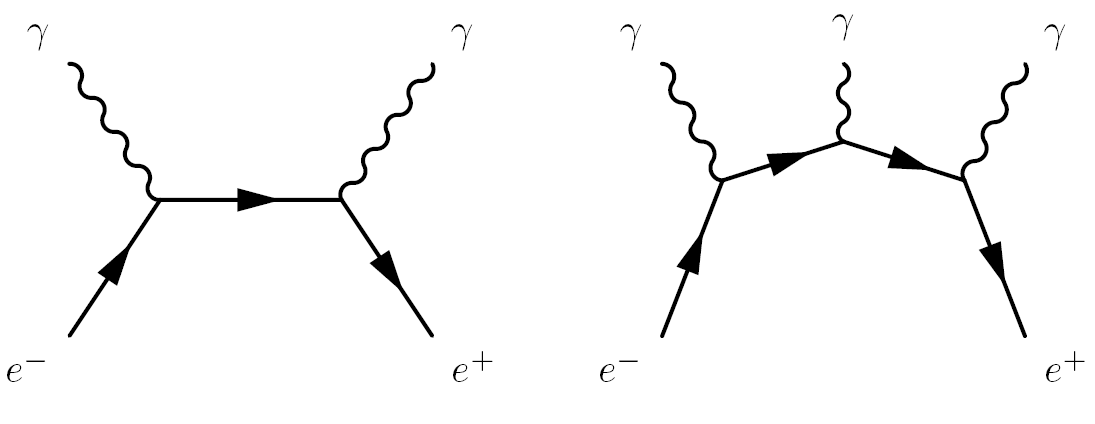
\includegraphics{feynman_positroniumdecay} \\
	\caption{Feynman Diagrams of the Annihilation processes of a positron with an electron (from the surrounding material of from the bound state in positronium),taken from \cite{Lab_manual_T8}. In presence of a nucleus which absorbs an outgoing photon, the annihilation to one photon is possible as well (suppressed).}
	\label{fig:feynman_positronium}
\end{figure}


\chapter{Experimental Setup}

The measurement of the lifetime is based on the property of the positron source $\isotope[22]{Na}$ which emits nearly instantaneously a photon in the subsequent decay ($\isotope[22]{Ne}^*\rightarrow \isotope[22]{Ne} $). The idea is to use this gamma ray with an energy of $E = \SI{1.2}{\mega\electronvolt}$ as start signal for the time measurement and one of the photons from the positron annihilation as stop signal ($E=\SI{511}{\kilo\electronvolt}$). The high energy photons are detected with plastic scintillators where they mostly create a high energy compton electron which subsequently produces scintillation light. Next to the scintillators on each side of the sample, two photomultiplier tubes (PMTs) are installed where the scintillation photons are converted to an electrical signal. The PMTs provide two signals: One at the last dynode and finally an integrated signal from the anode. The detector setup is schematically shown in figure \ref{fig:positron_setup}. Additional to one \isotope[22]{Na} source in Aluminum and one in Polyethylen, a \isotope[60]{Co} source (two coincident $\gamma$) is used to measure the resolution of the experimental setup. Furthermore, the two detectors can be replaced by a pulse generator for time calibration.

\begin{figure}
	\centering
	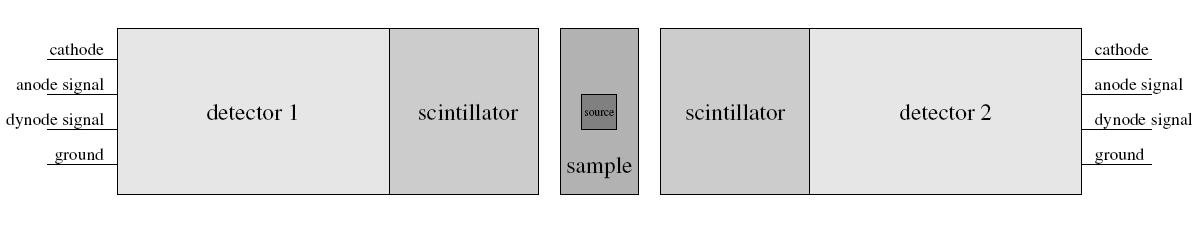
\includegraphics{positron_setup}
	\caption{Scheme of the experimental setup, taken from \cite{Lab_manual_T8}.}
	\label{fig:positron_setup}
\end{figure}

The two signals from each PMT are processed in a coincidence circuit which consists of different modules to reject background. The full electrical circuit is shown in figure \ref{fig:full_circuit}. The processing of the anode signal consists of the following steps (outer lines): At first, the signals are amplified. To reject background, the signal height is afterwards compared to a threshold in a Constant Fraction Discriminator (CFD) which provides a NIM-pulse and prevents 'time walk'\cite{Lab_manual_T8}. The actual measurement of the time difference between the start and the stop photons takes place in the Time Amplitude Converter (TAC) which charges a capacitor for the time between the two signals and delivers a pulse after discharging over a resistor. Finally, the pulse height is analyzed in a Multi Channel Analyzer module (MCA) and filled in a histogram. Parallel to this, the signals from the last dynode are processed and used to tune the setup for the photons of interest: The dynode signal is proportional to the energy of the initial photon and can thus be used to reject events where the energy does not match the expectation. The signal processing after the two PMTs is therefore specialized: One circuit accepts signals as expected from the first initial photon ($\gamma$ from \isotope[22]{Ne}) and the other from the annihilation photons ($e^+e^- \rightarrow 2\gamma$). The adjustment of these energy windows which are accepted is described in section \ref{sec:PrepandCal}. If both dynode signals pass the Window Discrimators (WD), they are used as coincidence signal and trigger the gate of the MCA. Only in this case, the pulse from the TAC is filled in the histogram. 

\begin{figure}
	\centering
	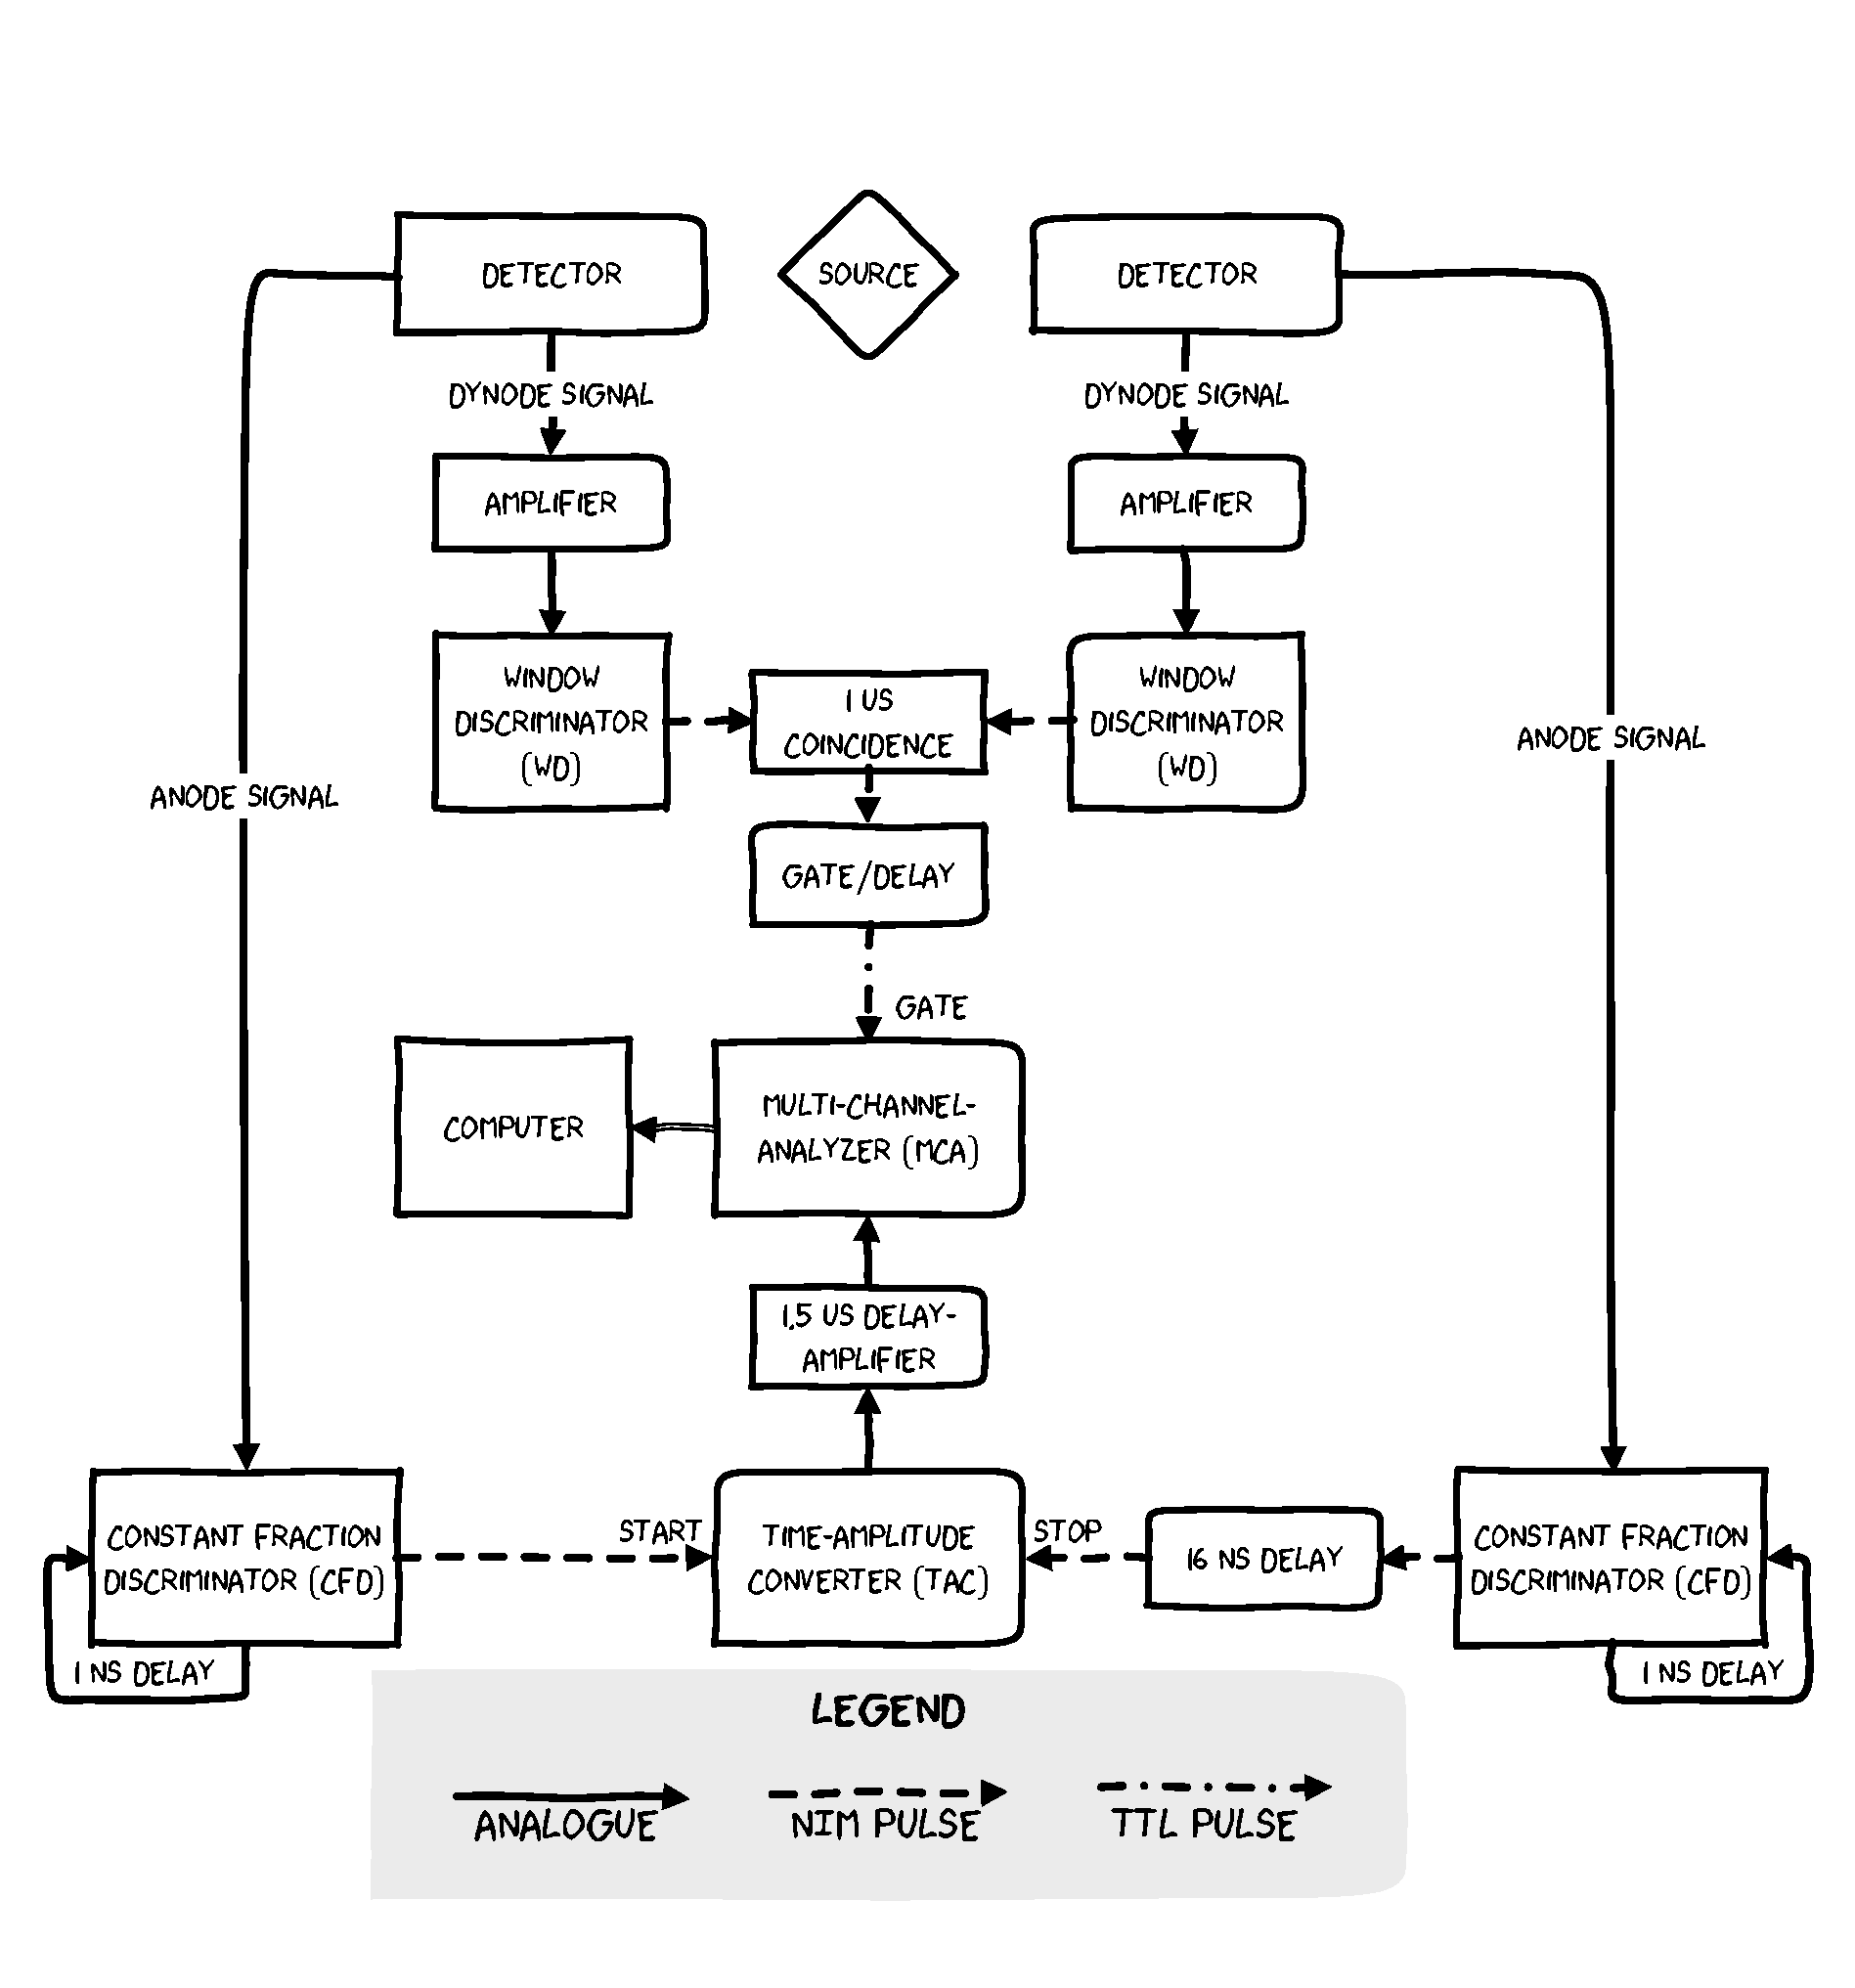
\includegraphics{aufbau}
	\caption{Full electrical circuit showing the processing of the two anode and dynode signals. The outer lines describe the steps of the anode signals which result in the time-measurement with the TAC and MCA. The inner lines show the processing of the dynode signals which are used to reject events which do not match the energy expectation of the start or stop photons.}
	\label{fig:full_circuit}
\end{figure}


\chapter{Preparation and Calibration of the Setup}
The setup as presented in the last chapter has to be adjusted to optimize the background rejection and to synchronize the delay of different parts of the full electrical circuit. These adjustment steps and the final time calibration with a pulse generator are presented in this chapter.
\section{Adjustment of the Window Discriminators}

To choose the window of accepted energies (dynode signal height), the circuit of the dynode is altered such that the MCA measures the energy spectrum of the detected photons, see figure \ref{fig:WD_circuit}. If the amplitude of the amplified dynode signal passes the window discrimator, the value is analyzed and added to the energy spectrum. 
 
\begin{figure}[h]
 	\centering
 	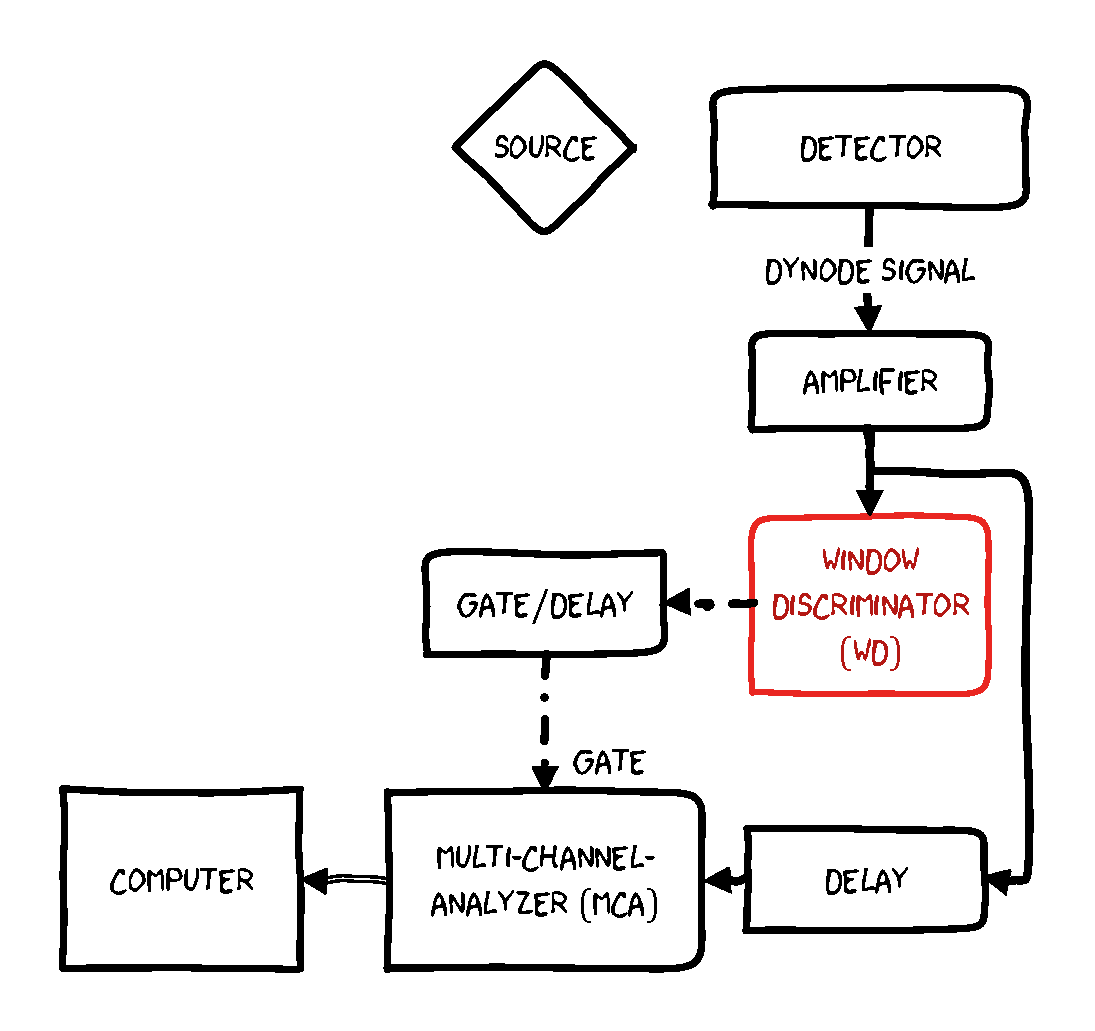
\includegraphics[width=0.7\textwidth]{aufbau_wd}
 	\caption{Altered circuit of one dynode signal to adjust the window discriminator.}
	\label{fig:WD_circuit}
\end{figure}
 
If the discrimination is disabled, the energy spectrum shows the typical form expected for a scintillation detector with the two characteristic Compton edges. The WD of the start circuit has to be tuned to the high energy photon and the WD of the stop circuit to the annihilation photons. The windows are therefore chosen around the corresponding Compton edges. The choice of parameters for the window discriminators are listed in table \ref{tbl:WD_values} and the resulting spectra are presented in figure \ref{fig:WD_spectra}. The values are not adjusted very tight because following measurements with a Cobalt source have to be conducted with the same setup.

\begin{table}[htbp]
	\centering
	\begin{tabular}{ 
			l
			l
			l
			l
		}
		\toprule
		{Circuit} & {Threshold} & {Window} & {Time Constant} \\ 
		\midrule
		Start & $185$ & $450$ & $\SI{1}{\micro\second}$ \\
		Stop & $0$ & $280$ & $\SI{1}{\micro\second}$ \\
		\bottomrule
	\end{tabular}
	\caption{Adjusted parameters of the two Window Discriminators, one tuned for the start photon and the other for the annihilation photons.}
	\label{tbl:WD_values}
\end{table}

\begin{figure}[h]
	\centering
	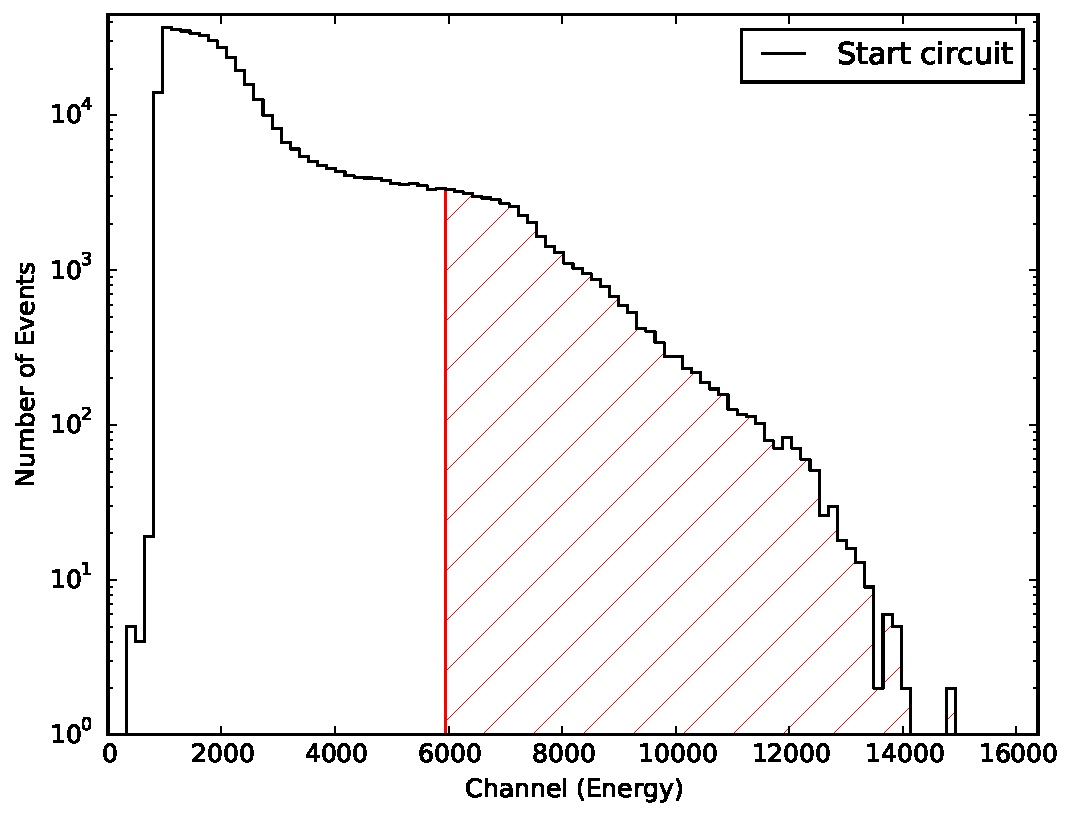
\includegraphics[width=0.8\textwidth]{windows_0}
	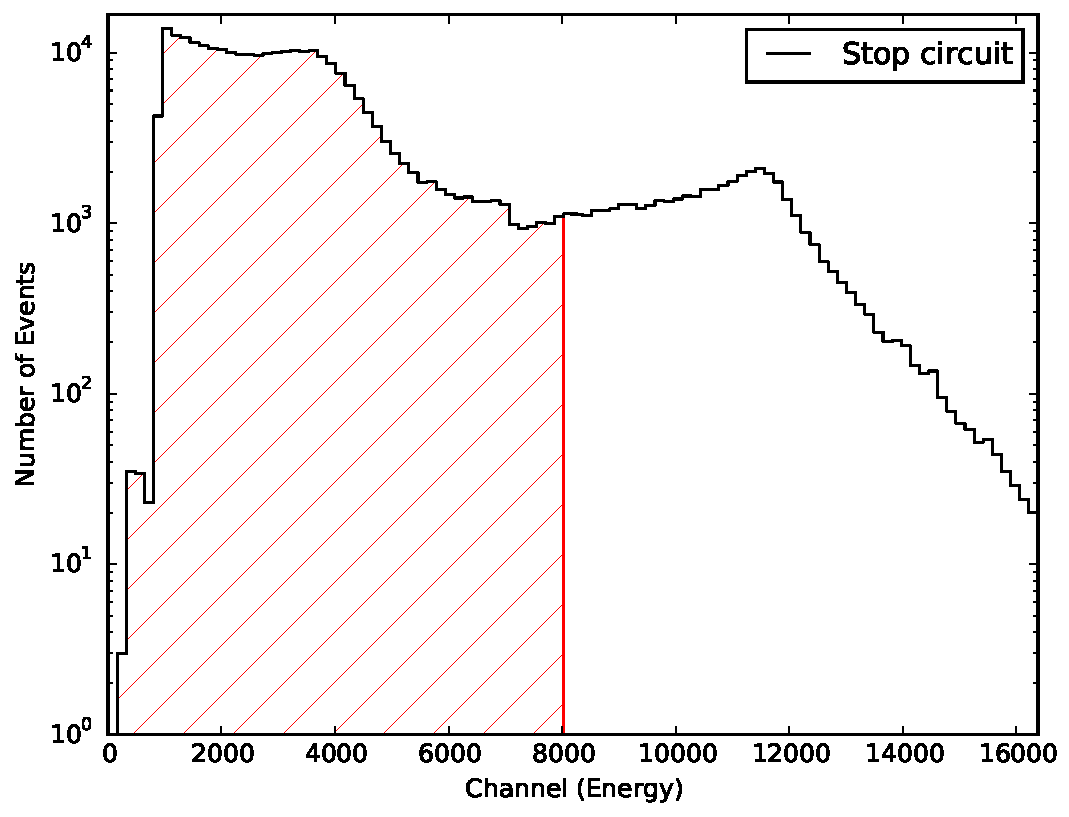
\includegraphics[width=0.8\textwidth]{windows_1}
	\caption{Energy spectra (uncalibrated) of the dynode signals in the start and stop circuit. The chosen windows are shown dashed.}
	\label{fig:WD_spectra}
\end{figure}

\FloatBarrier
\section{Adjustment of the Constant Fraction Discriminators}

In the processing of the anode signals, Constant Fraction Discriminators are used to reject background and noise. The threshold, Upper Level Discriminator and Lower Level Discriminator values are adjusted while the full electrical circuit is set up but no radioactive source is present between the scintillators: It is increased until the rate of misleadingly accepted events (energy windows passed, coincident and CFDs passed) becomes very low. The parameters are listed in table \ref{tbl:CFD_values}.

\begin{table}[htbp]
	\centering
	\begin{tabular}{ 
			l
			l
			l
			l
		}
		\toprule
		{Circuit} & {Threshold} & {ULD} & {LLD} \\ 
		\midrule
		Start & $45$ & $950$ & $160$ \\
		Stop & $145$ & $960$ & $140$ \\
		\bottomrule
	\end{tabular}
	\caption{Adjusted parameters of the two Constant Fraction Discriminators, tuned such that the rate of misleadingly accepted events is very low.}
	\label{tbl:CFD_values}
\end{table}

\section{Synchronization of the Gate and the TAC Signal}
An important parameter of the full electrical circuit is the timing between the gate-signal and the signal from the Time Amplitude Converter. The MCA accepts the pulse from the TAC only if the gate is already open. To adjust this timing, the two signals are investigated with an oscilloscope. The pulse of the TAC runs through a microsecond-delay because the energy circuit (dynode signals) is much slower. The synchronization is finally achieved by extending and delaying the gate signal in the Gate/Delay-module. The result is shown in figure \ref{fig:GateDynode_sync}.

\begin{figure}[h]
	\centering
	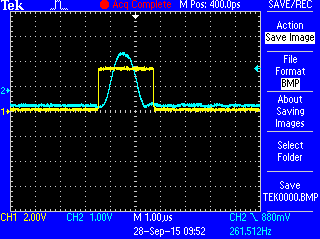
\includegraphics[width=0.7\textwidth]{../images/gate_vs_dynode/F0002TEK.png}
	\caption{Snapshot from the oscilloscope showing the synchronized signals from the Gate (yellow) and TAC(cyan).}
	\label{fig:GateDynode_sync}
\end{figure}

\FloatBarrier
\section{Time Calibration and Determination of the Electronic Resolution}
The goal of this calibration experiment is to map the MCA channels to a physical delay between the PMT signals. 

To simulate realistic conditions, the experimental setup is very similar to the one depicted in figure \ref{fig:full_circuit}. The only  exception is that the detectors as well as the radioactive source are replaced by a digital pulse generator. The pulse generator is configured such that the pulse heights and lengths resemble the signals from the PMTs.  
The delay is manually entered into the pulse generator, delaying the stop circuit. A delay range of \SIrange{0}{20}{\nano\second} is sampled in \SI{1}{\nano\second} steps, additional points at \SI{25}{\nano\second} and \SI{30}{\nano\second} are recorded.

\begin{sidewaysfigure}
	\centering
	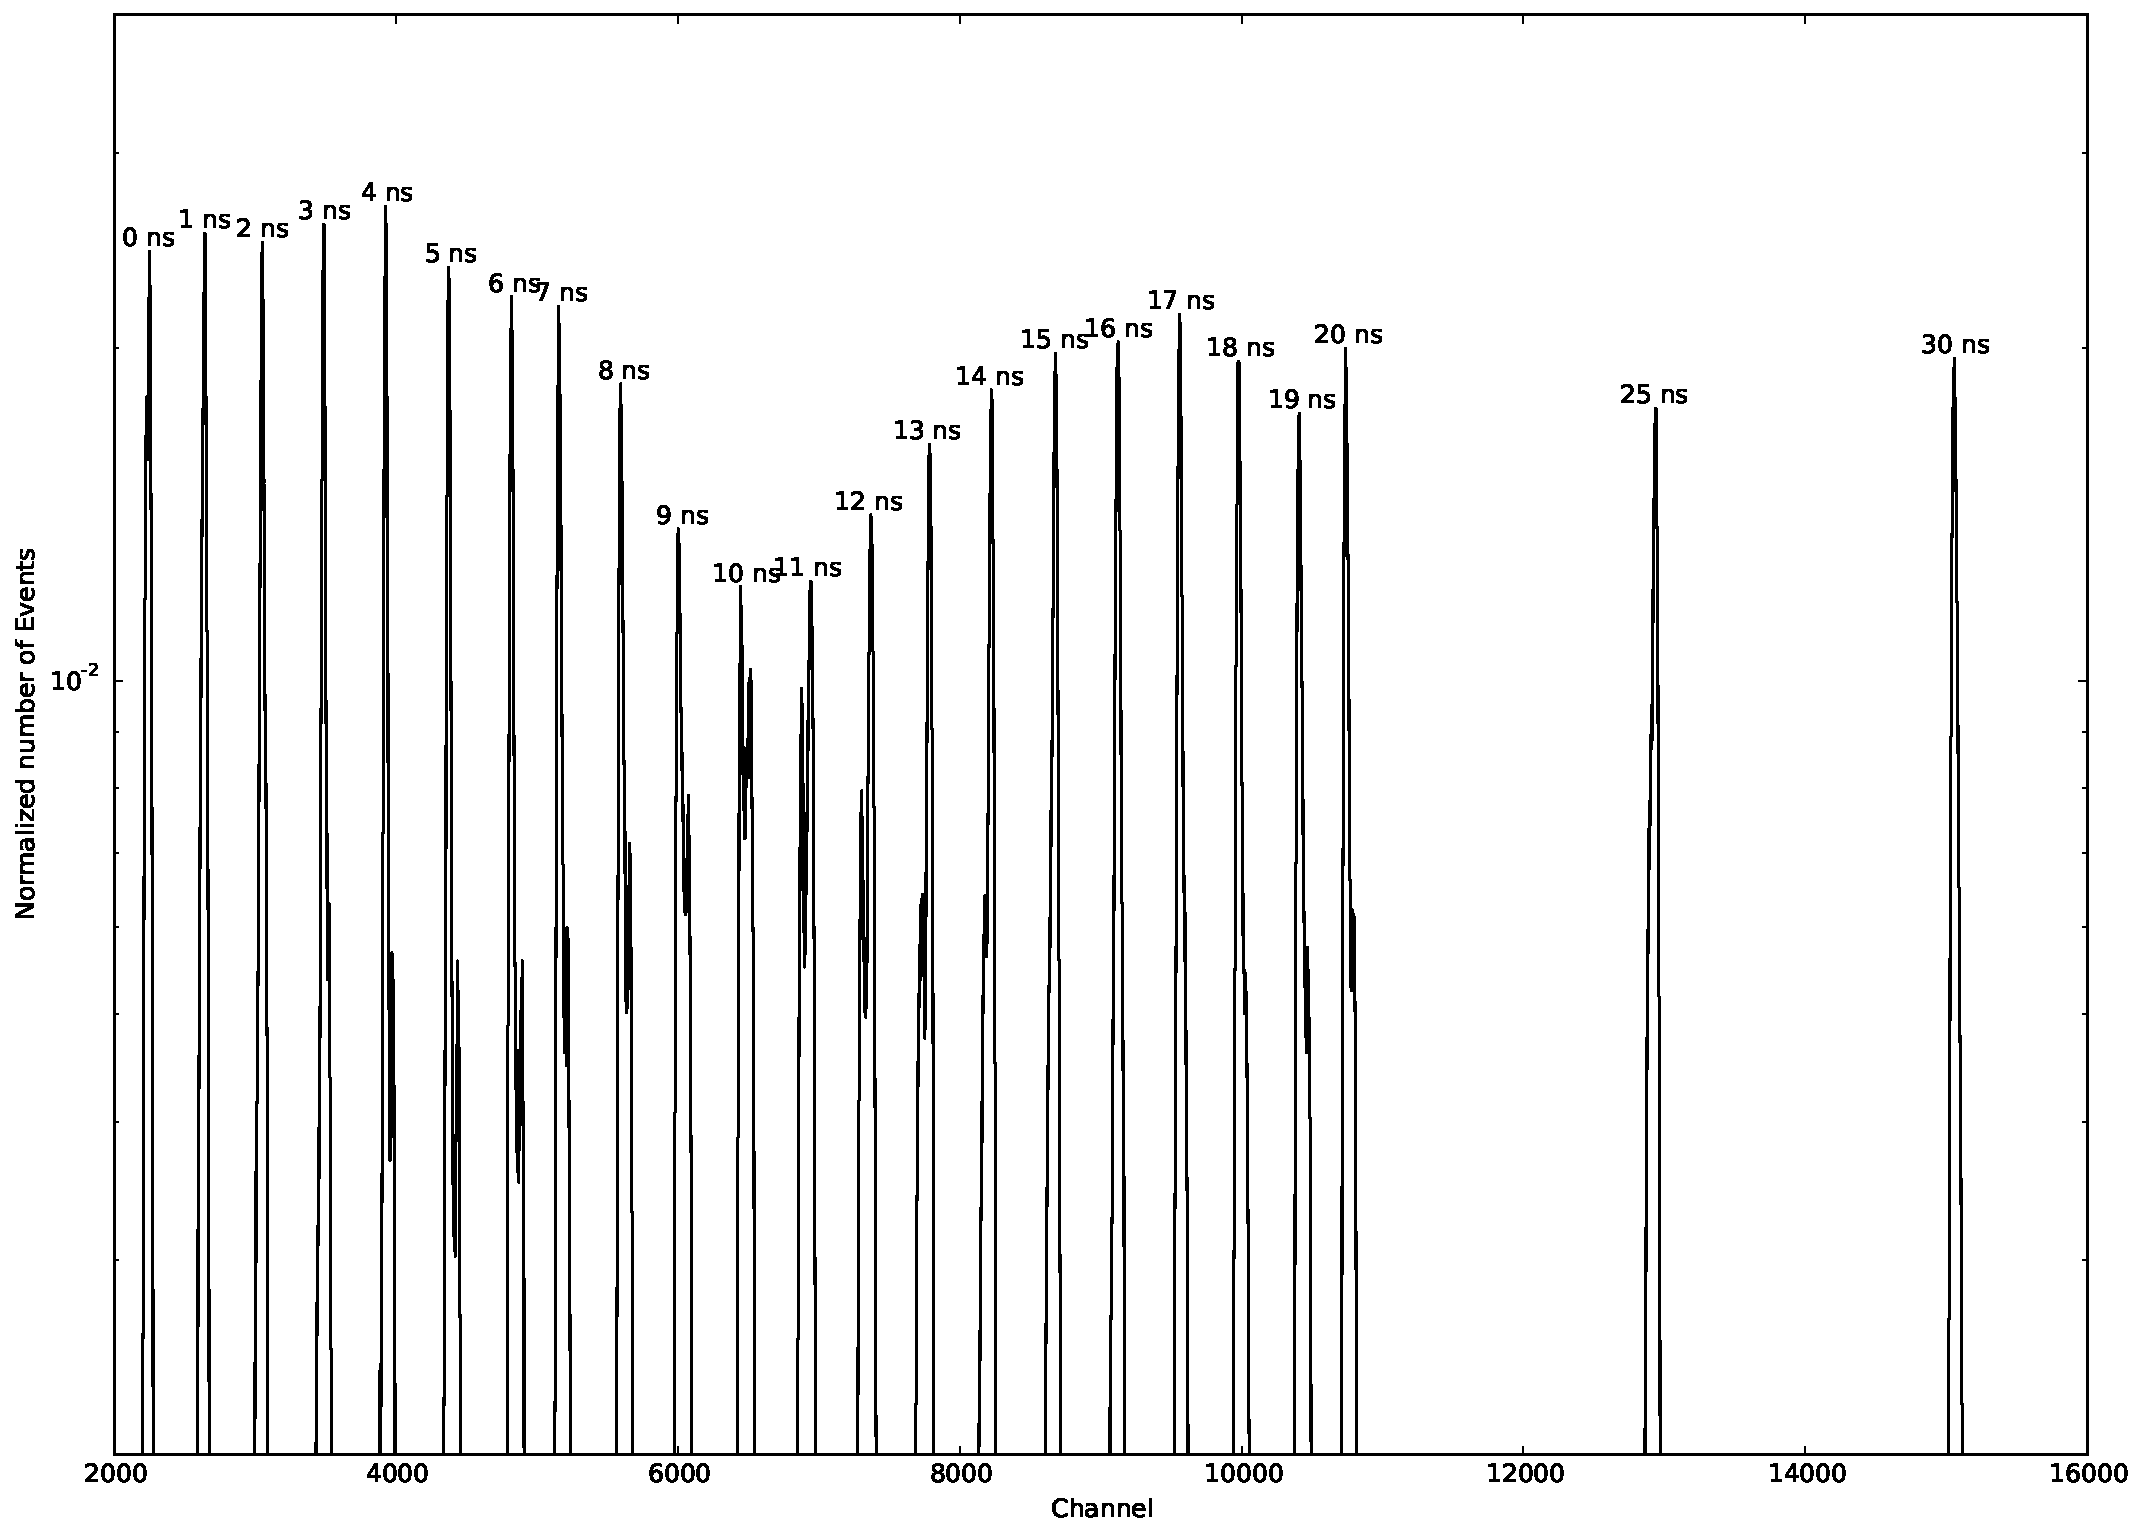
\includegraphics{calibration_peaks}
	\caption{Peaks of the time calibration. Each peak has been normalized to an area of \num{1}.}
	\label{fig:calibration_raw}
\end{sidewaysfigure}

The measured data is shown in figure \ref{fig:calibration_raw}. As expected, the measurements show up as narrow equidistant peaks. Each peak has been normalized to contain \num{1} event in total. This way the peak shapes can be compared. As one can easily see (especially around \SIrange{4}{13}{\nano\second}), the peaks are actually made up from two separate Gaussian curves. By exchanging modules from the experimental setup this behavior can be traced back to the \SI{16}{\nano\second} delay between the stop-circuit-CFD and the TAC. Replacing the module by a different delay does not mitigate the issue.

Since neither of the bumps is physically motivated, both will be considered in the calibration and the uncertainty adjusted accordingly.
First the extend of a peak is calculated. Around a manually entered seed, the maximal bin value is calculated. All adjacent bins with more than \SI{2}{\percent} of the maximum value are assumed to belong to the peak. From the entire range, the centroid is calculated. This is the center value $\bar{x}$ of the curve. Symmetrically around the center value $\bar{x}$, a region from $\bar{x}-\sigma_x$ to $\bar{x}+\sigma_x$ is defined. $\sigma_x$ is initially set to \num{0}, but then increased until the integral of the region contains \SI{68}{\percent} of the total peak value ($ = \num{1}$). The value $\sigma_x$ can then be interpreted as uncertainty, analogous to the standard deviation of a Gaussian distribution.

Each peak is now characterized by a delay time $\Delta t$, a center channel value $\bar{x}$ and a peak uncertainty $\sigma_x$.
A linear regression is performed on this data. Using $\chi^2$ minimization, the parameters of $f(x) = a x + b$ are optimized. 
The uncertainty of the parameters is determined by simulating "pseudo-experiments": \num{1000} times, all data points are chosen from a normal distribution around their measured value with their uncertainty. The fit is performed for each pseudo-experiment, mean and standard deviation of the fit result yield the final value and uncertainty on the fit parameters.

\begin{figure}
	\centering
	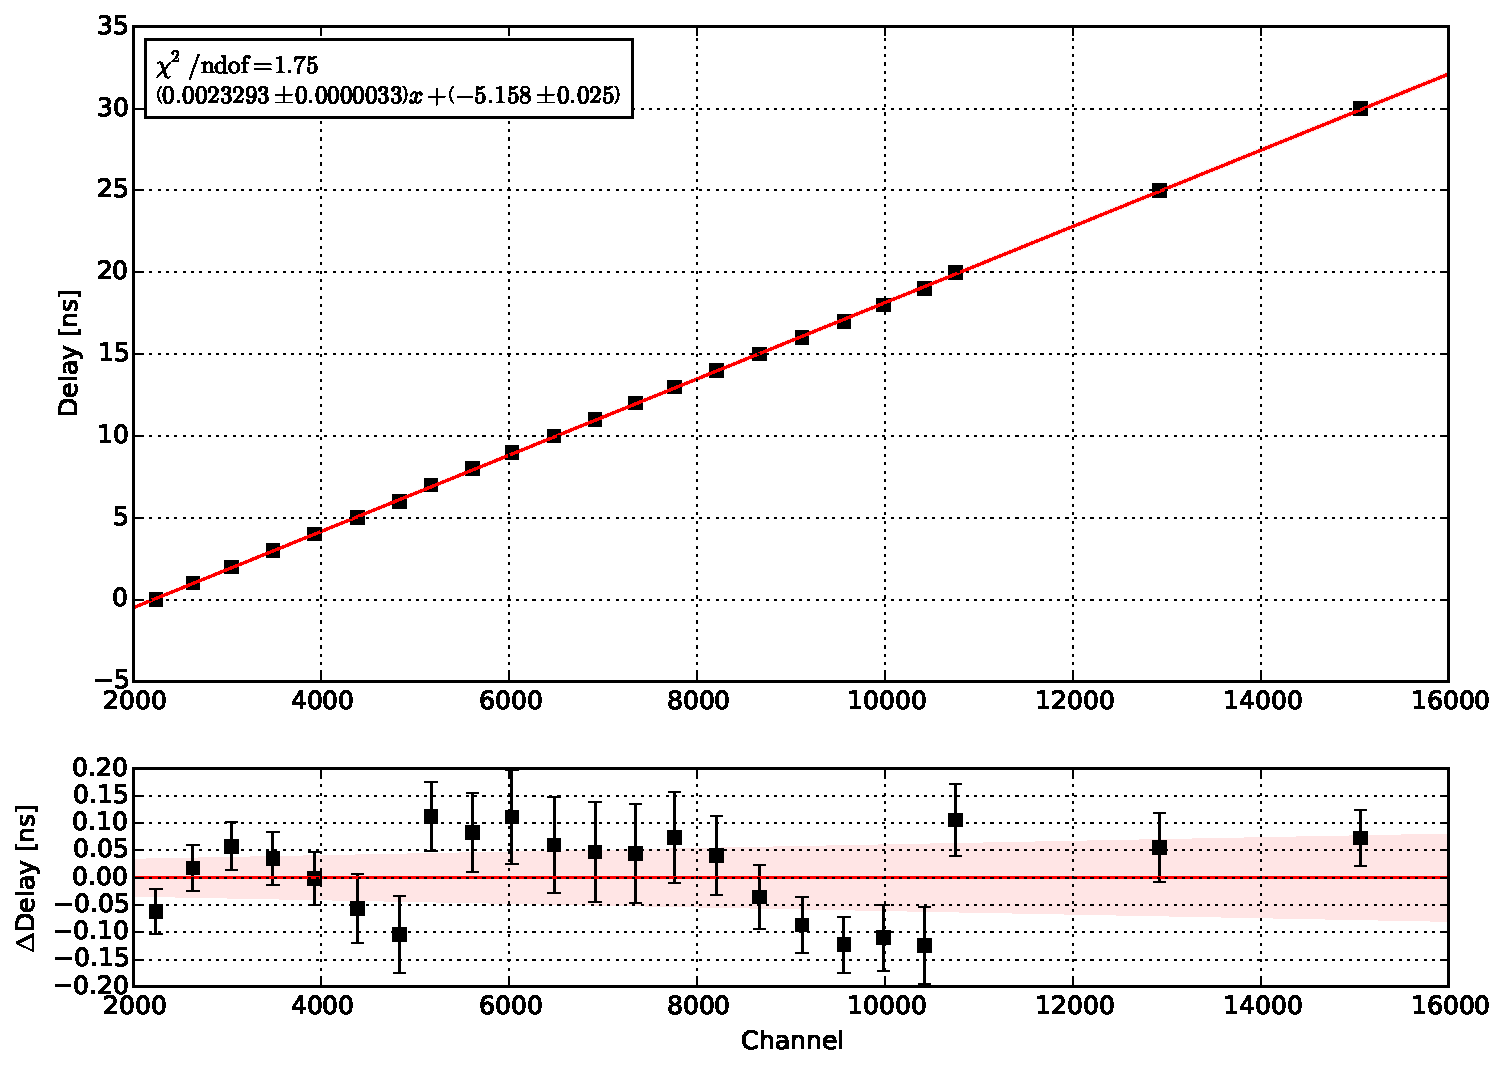
\includegraphics{calibration}
	\caption{Linear regression result.}
	\label{fig:calibration_linreg}
\end{figure}

The regression result with the residuum is depicted in figure \ref{fig:calibration_linreg}. The residuum plot on the bottom contains the channel uncertainty projected onto the fitted function. Despite a small visible systematic deviation in the residuum plot, $\chi^2/\mathrm{ndof} = 1.74$ indicates that the fitted model describes the data. This explicitly justifies the choice of the delay-value in the stop-circuit since TAC and MCA seem to operate in a linear region.

The final calibration function is
\begin{equation}
	\Delta t = \left[\left(\num{0.0023292 \pm 0.0000034}\right) \cdot \mathrm{channel} + \left(\num{-5.163 \pm 0.025}\right)\right] \si{\nano\second}
\end{equation}

This result can be combined with the mean and sample standard deviation of the obtained peak widths to calculate the time resolution due to electronics:
\begin{equation}
	\sigma_{t,\mathrm{elec}} = \SI{64.4 \pm 15.5}{\pico\second}
\end{equation}

\chapter{Conduction and Analysis}
The presented experimental setup results in a measurement of time differences between the start and stop photons from the source. It is conducted with three different sources: \isotope[22]{Na} in Aluminum, \isotope[22]{Na} in Polyethylen and \isotope[60]{Co} in Polyethylen. The first two measurements aim to determine the lifetime/conversion time of positrons in metals and plastic and the third source provides two coincident photons which are investigated to determine the time resolution of the setup. Furthermore, the \isotope[60]{Co} source is used to investigate the stability of the setup by comparing the corresponding histogram before and after a measurement with another source.

\begin{table}[htbp]
	\centering
	\begin{tabular}{ 
			l
			l
		}
		\toprule
		{Source} & {Measurement Time}  \\ 
		\midrule
		\isotope[60]{Co} in Plastic  & $\SI{5880}{\second}$  \\
		\isotope[22]{Na} in Aluminum & $\SI{43620}{\second}$  \\
		\isotope[22]{Na} in Plastic  & $\SI{246900}{\second}$ \\
		\bottomrule
	\end{tabular}
	\caption{Duration of the different measurements.}
	\label{tbl:Meas_times}
\end{table}



\section{Rebinning of Histograms and Background Subtraction}
All following analysis steps are based on the measured numbers of events per channel in the MCA. The number of bins in the investigated histograms (frequency of occurred delays) is chosen smaller than the number of channels in the MCA($\approx 16000$). The reason lies in the number of events per bin which is requested for the interesting regions to be larger than $\approx 20$. This justifies poissonian error estimation $\sigma_\textrm{bin}=\sqrt{n_\textrm{bin}}$ during fit procedures. \\

Even though the experimental setup is tuned to reject background events, there is a certain fraction of events which do not come from actual positrons (noise in the PMT, natural radioactivity etc.). The random time between two background signals follows a uniform distribution. In all histograms, the tail corresponding to very large time differences is therefore investigated to determine the constant background: The procedure is exemplary shown in figure \ref{fig:resolution_background}(blue line) where the background is estimated in the range \SIrange{20}{30}{\nano\second} and then subtracted in all bins of the histogram. 

\begin{figure}
	\centering
	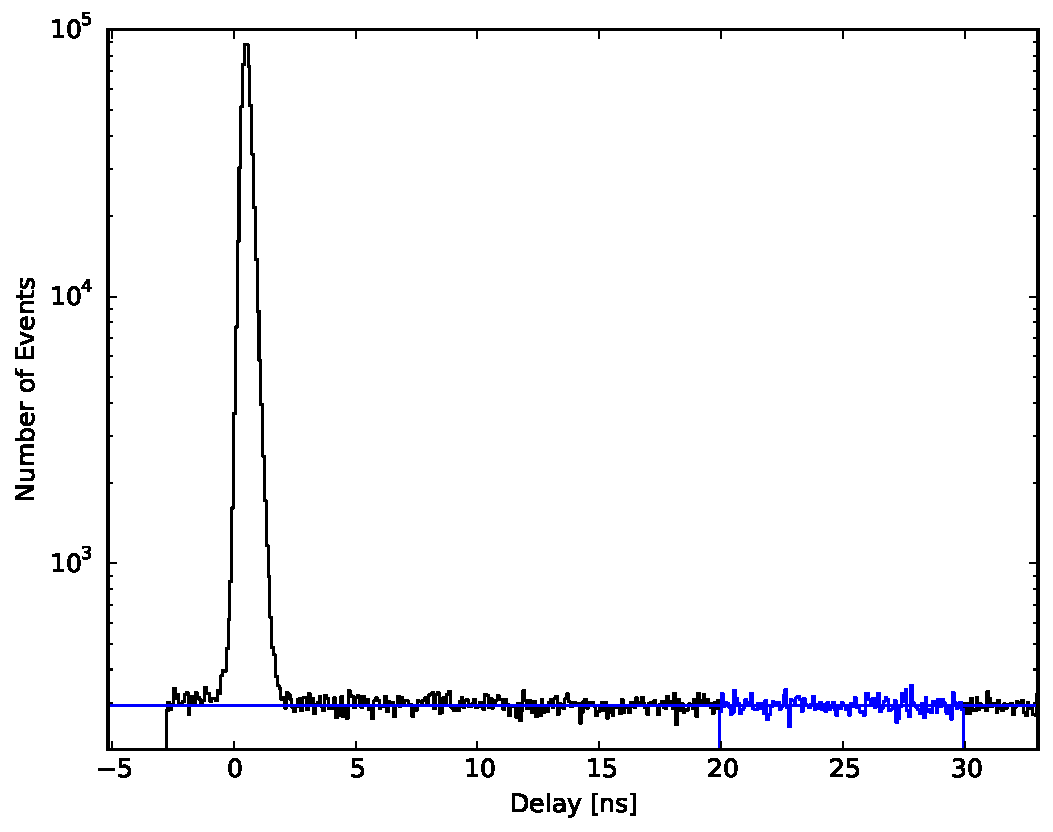
\includegraphics{resolution_background}
	\caption{Demonstration of the Background Subtraction process which is applied in all following histograms.}
	\label{fig:resolution_background}
\end{figure}

\section{Determination of the Full Time Resolution}
The \isotope[60]{CO} source provides two coincident high energy photons which can be used to investigate the resolution of the full setup (time calibration used a setup excluding the detectors). It is placed between the scintillators and the time difference of the actually coincident photons is measured. The resulting histogram can be seen in figure \ref{fig:resolution_peak}. 

\begin{figure}
	\centering
	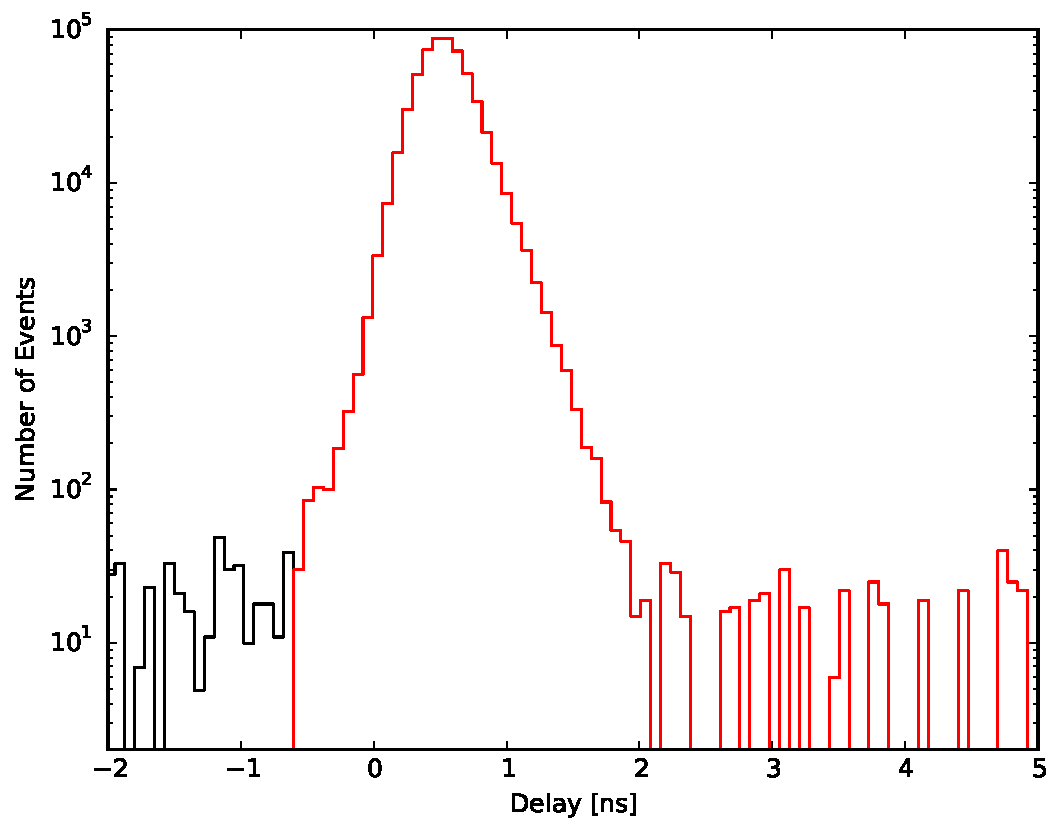
\includegraphics{resolution_peak}
	\caption{Determination of the Resolution Curve of the full setup using \isotope[60]{Co}.}
	\label{fig:resolution_peak}
\end{figure}

The time resolution of the full setup can now be obtained from a fitted Gauss function. The fit shows deviations to larger delay times (asymmetry in the tail) and the $\chi^2$ value does not match the expectation. However, in a wide range around the peak, the curve can be described well by a Gaussian function and the result can be used as estimate for the resolution (no error is stated becaus of the described fit issues):

\begin{equation}
	\sigma_{t,full}=\SI{283}{\pico\second}
\end{equation}

\section{Lifetime/Conversion Time in Plastic}

\section{Short Positronium Lifetime in Aluminum}

The first measurement of the positron lifetime with the \isotope[22]{Na} in Aluminum is conducted over night (livetime stated in table \ref{tbl:Meas_times}). The resulting histogram showing the frequency of occurred time differences is presented in figure \ref{fig:Na22_alu}. 

\begin{figure}
	\centering
	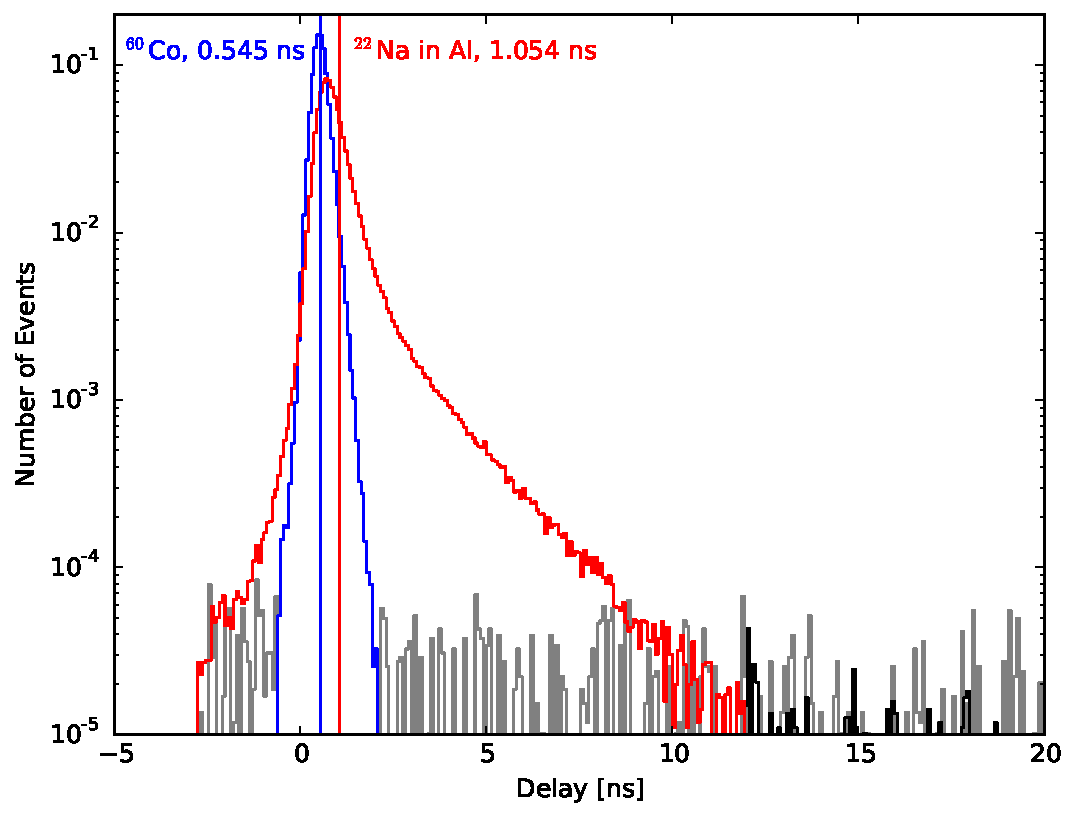
\includegraphics{na22_aluminum}
	\caption{Histogram of occurred delays between the start and stop signal. The measurement of \isotope[22]{Na} in aluminum (red) is shown together with the resolution curve (blue). The vertical lines show the centroids of the colored ranges.}
	\label{fig:Na22_alu}
\end{figure}

The expected lifetime of positrons in aluminum (no positronium formed in metal) is much smaller than the resolution of the presented setup. However, a measurement of this quantity is possible by the so called 'centroid-shift-method'. Assuming a model with an exponential decay and the convolution with a resolution curve, the decay constant can be extracted from the difference of the centroids \cite{Lab_manual_T8}:
\begin{equation}
	\tau = \frac{1}{\lambda} = \frac{\sum_i t_i N_{\textrm{Meas},i}}{\sum_i N_{\textrm{Meas},i}} - \frac{\sum_i t_i N_{\textrm{Res},i}}{\sum_i N_{\textrm{Res},i}} 
\label{eq:centroid}
\end{equation}

In equation \ref{eq:centroid}, $N_x$ is the number of entries in one bin and $t_x$ stands for the delay which corresponds to this channel. The centroid of the measured curve of \isotope[22]{Na} (blue vertical line in figure \ref{fig:Na22_alu}) is shifted compared to the centroid of the resolution curve (red vertical line same figure). This method gives the following result for the lifetime of positrons in aluminum (error obtained from the standard deviation of both centroids propagated to the shift result):
\begin{equation}
	\tau_\textrm{alu}= \left( 510 \pm 10 \right) \si{\pico\second}
\end{equation}

\section{Deviation to the Expected Lifetime in Metal}

The expectation for the lifetime of positrons in metals was stated in chapter \ref{ch:theory} in the \si{\pico\second} regime. The measured result is not compatible with this expectation. A suspicious observation is that the decay constants of the measurement in aluminum and plastic are very similar. It is thus not surprising that the centroid shift which aims for 



\chapter{Systematic Uncertainties}

\chapter{Results and Conclusion}


\cleardoublepage

\bibliographystyle{utphys}
\bibliography{T8_bib}{}

\end{document}


